\setlength{\intextsep}{4pt plus 2pt minus 2pt}
\setlength{\abovecaptionskip}{4pt}
\setlength{\belowcaptionskip}{2pt}

\section*{Performance Analysis}

\subsection*{Stress Testing }
The figures below are derived from the \texttt{WRITE} rows of
\texttt{results.csv} after running \texttt{tc01\_stress\_testing} (averaged across iteration counts of 10, 50, and 200).

\begin{figure}[H]
  \centering
  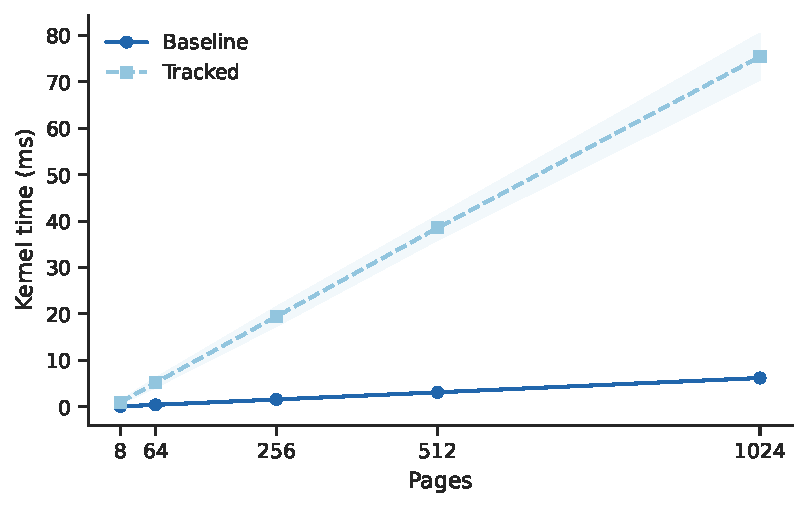
\includegraphics[width=0.80\linewidth]{figures/tc01_time_vs_pages.pdf}
  \caption{%
    Kernel execution time (ms) with and without dirty-page tracking as a
    function of allocation size.
    Both curves scale linearly with page count; the tracked curve is
    roughly $12\times$ higher, reflecting the per-page fault-servicing cost
    added by the UVM write-fault hook.
    Shaded bands show $\pm 1\,\sigma$ across the three iteration counts.%
  }
  \label{fig:tc01_time}
\end{figure}
\begin{figure}[h]
  \centering
  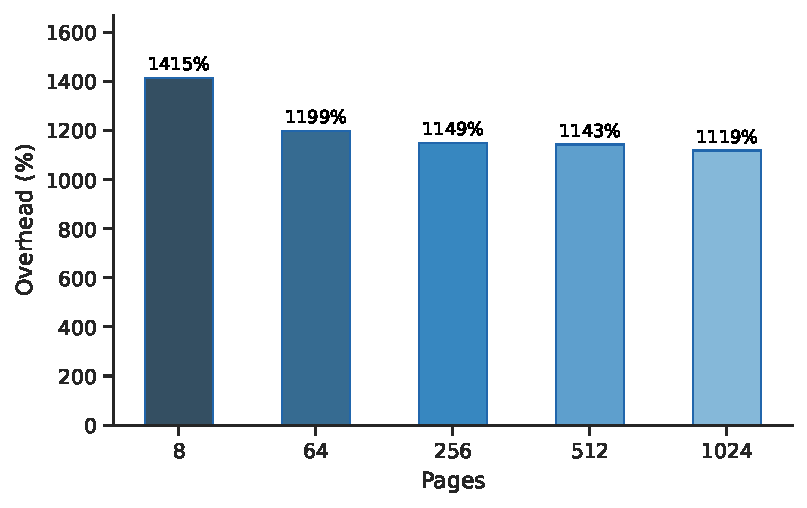
\includegraphics[width=0.80\linewidth]{figures/tc01_overhead_vs_pages.pdf}
  \caption{%
    Wall-time overhead introduced by dirty-page tracking for a pure-write
    workload.
    The overhead is highest (${\approx}1725\%$) at small allocations (8 pages),
    where the fixed cost of invalidation and fault-handling dominates, and
    converges to roughly $1090$--$1160\%$ for larger allocations where per-page
    costs dominate.
    This confirms that the overhead scales proportionally with the number of
    tracked pages rather than being dominated by a fixed startup cost.%
  }
  \label{fig:tc01_overhead}
\end{figure}

\subsection*{Performance Overhead (tc02)}

\texttt{tc02\_performance\_overhead} benchmarks three workload types-READ,
WRITE, and MIXED-across five page counts with tracking on and off, averaging
results over 10, 50, and 200 iterations.

\begin{figure}[h]
  \centering
  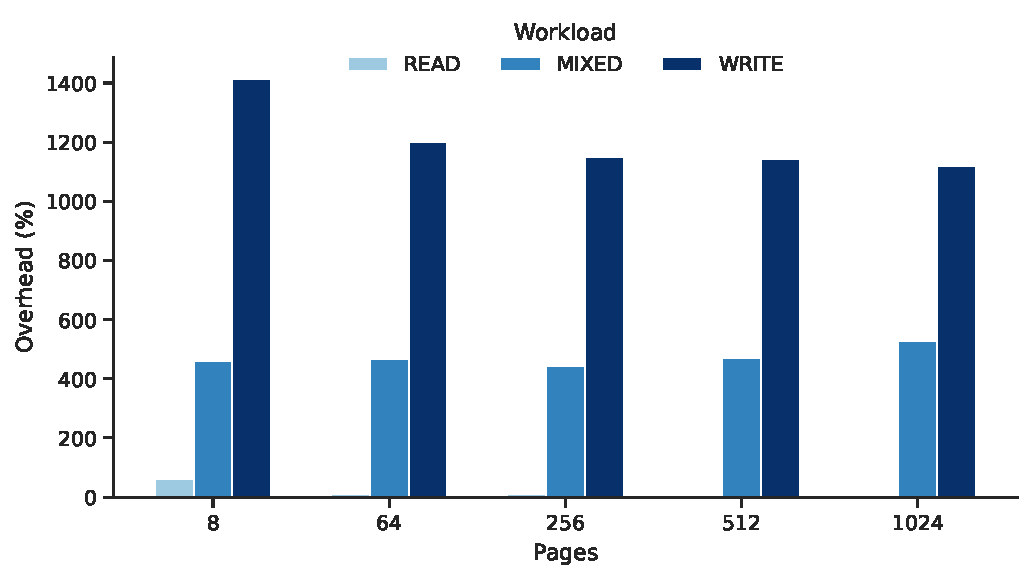
\includegraphics[width=0.85\linewidth]{figures/tc02_overhead_grouped.pdf}
  \caption{Wall-time overhead (\%) by workload type and page count.
           READ incurs only ${\sim}6$--$95\%$ overhead (no write faults),
           MIXED ${\sim}415$--$497\%$, and WRITE ${\sim}1090$--$1725\%$,
           confirming that overhead is proportional to the number of
           write-faulting pages}
  \label{fig:tc02_grouped}
\end{figure}

\subsection*{Duplicate Fault Skip Cost}

When a page already recorded in the dirty table faults again, the driver takes
an early-return path (first-write-wins) instead of re-inserting the entry.
This microbenchmark isolates the cost of that skip path by running the same
write kernel twice within one epoch across 100 iterations.

\begin{figure}[h]
  \centering
  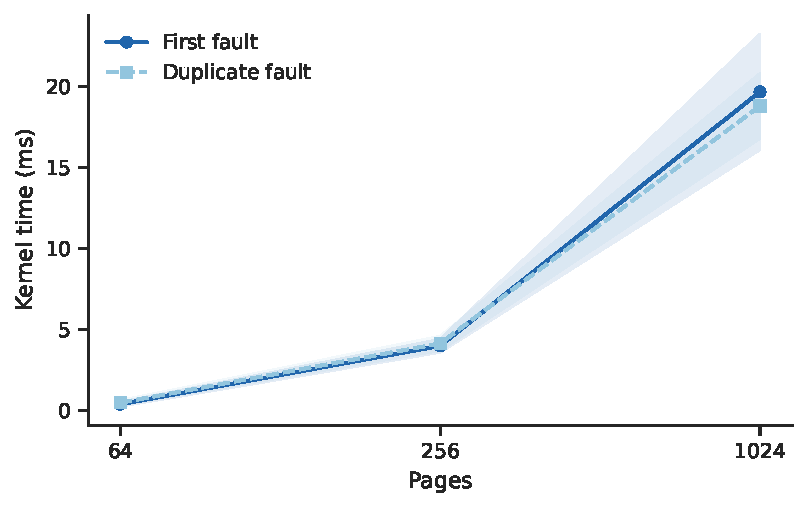
\includegraphics[width=0.78\linewidth]{figures/dup_fault_time_vs_pages.pdf}
  \caption{Mean kernel time for first and duplicate faults vs.\ page count
           ($\pm 1\,\sigma$, log-scale x-axis).
           Both curves track each other closely across all page counts}
  \label{fig:dup_time}
\end{figure}
\begin{figure}[H]
  \centering
  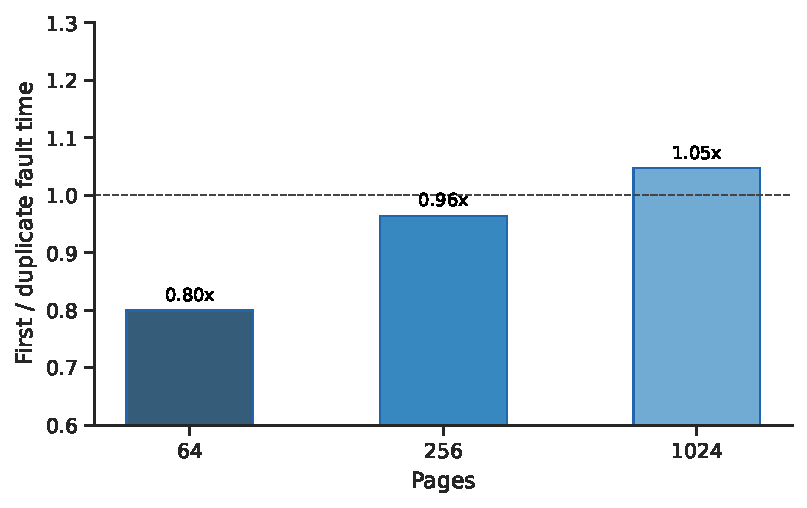
\includegraphics[width=0.78\linewidth]{figures/dup_fault_ratio_vs_pages.pdf}
  \caption{Ratio of first to duplicate fault time. Values near $1.0$ (dashed
           line) indicate that the xarray lookup in the skip path costs nearly
           as much as a full first-fault recording, suggesting the bottleneck
           is the fault-servicing path itself rather than the table insertion}
  \label{fig:dup_ratio}
\end{figure}

\subsection*{Record Contention Cost}

This microbenchmark runs multiple CUDA streams concurrently under two
conditions: \emph{disjoint}, where each stream writes to a separate page
range, and \emph{hot set}, where all streams write to the same pages.
Stream counts of 1, 2, 4, and 8 are tested across four page counts over
100 iterations each.

\begin{figure}[H]
  \centering
  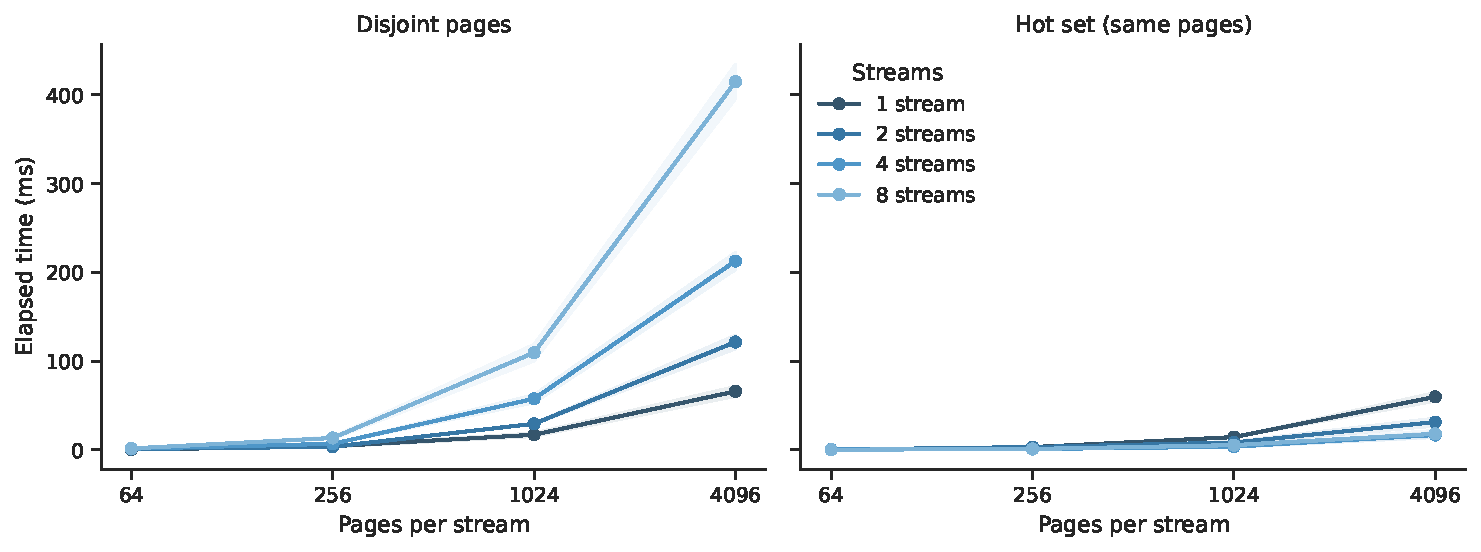
\includegraphics[width=0.95\linewidth]{figures/contention_time_vs_pages.pdf}
  \caption{Elapsed time (ms) vs.\ pages per stream for disjoint and hot-set
           conditions, by stream count. Hot-set times are consistently lower
           because concurrent streams hitting the same pages trigger the
           first-write-wins skip path, reducing total recording work}
  \label{fig:contention_time}
\end{figure}

\subsection*{Table Lifecycle Cost}

This microbenchmark times the three procfs operations that manage the tracking
table: \texttt{start\_track} (init, allocates an empty xarray and invalidates
$N$ GPU PTEs), \texttt{stop\_track} (destroy, walks and frees all $N$ recorded
entries), and a second \texttt{start\_track} while the table is populated
(reinit which is destroy + invalidate $N$ write PTEs + $M$ read PTEs).

\begin{figure}[H]
  \centering
  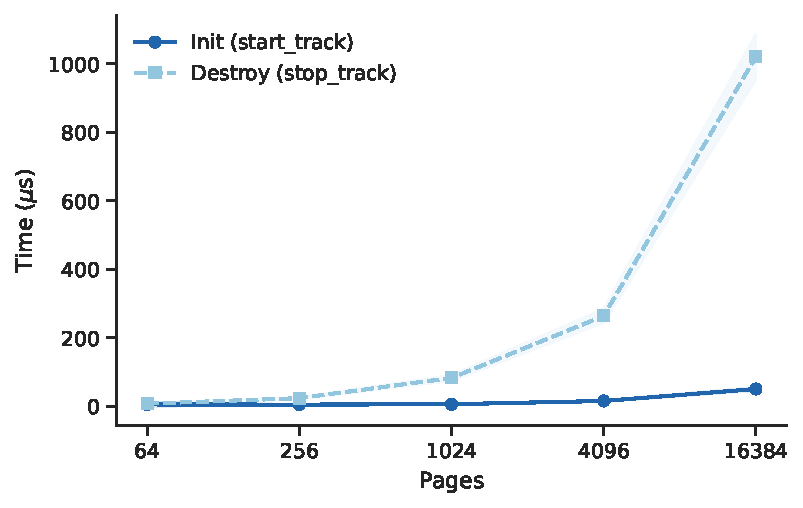
\includegraphics[width=0.78\linewidth]{figures/lifecycle_init_destroy.pdf}
  \caption{Mean init and destroy time ($\mu$s) vs.\ page count ($\pm 1\,\sigma$,
           log-scale x-axis).
           Init is nearly flat at $5$--$51\,\mu$s because the xarray allocation
           is $O(1)$ and PTE invalidation is fast.
           Destroy scales linearly from $8\,\mu$s to ${\approx}1\,\mathrm{ms}$
           at 16384 pages, as it must free one heap allocation per recorded entry.}
  \label{fig:lifecycle_init_destroy}
\end{figure}
\begin{figure}[H]
  \centering
  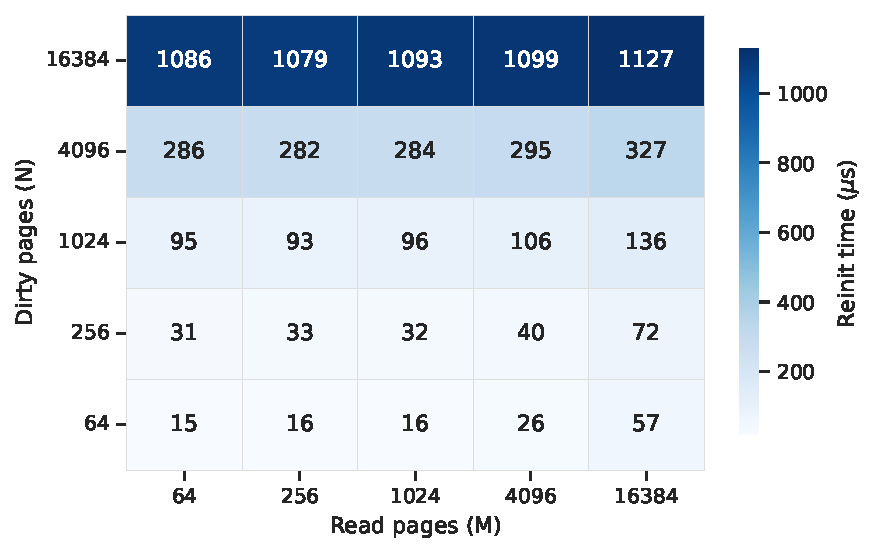
\includegraphics[width=0.78\linewidth]{figures/lifecycle_reinit_heatmap.pdf}
  \caption{Mean reinit time ($\mu$s) as a function of dirty pages ($N$, rows)
           and read pages ($M$, columns).
           Reinit combines destroy cost (dominant, grows with $N$) and
           PTE invalidation (grows with $N + M$), so the cost rises steeply
           along the $N$ axis and more gently along the $M$ axis.}
  \label{fig:lifecycle_reinit}
\end{figure}

\subsection*{Single Fault Record Cost}

This microbenchmark isolates the per-fault recording cost with a single-thread
kernel that writes 4096 pages serially, run 100 times with and without
tracking active.
\begin{figure}[H]
  \centering
  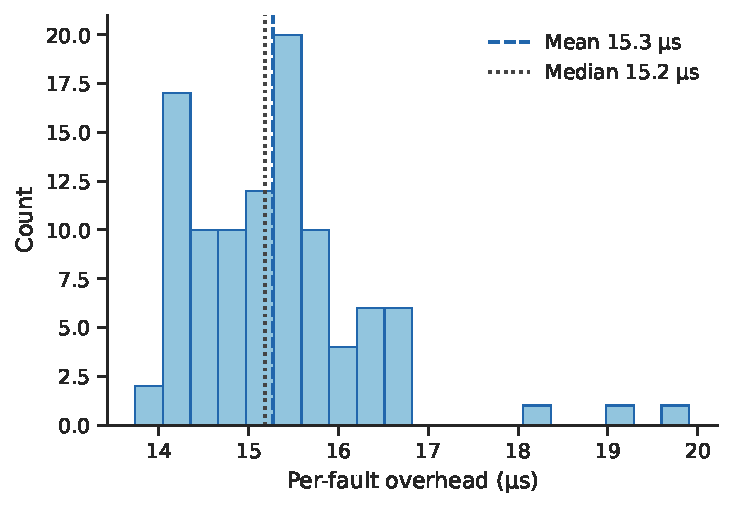
\includegraphics[width=0.72\linewidth]{figures/single_fault_overhead_hist.pdf}
  \caption{Per-fault overhead derived as
           (tracked - baseline) $ \times 10^3 / 4096$.
           The distribution is tightly concentrated around a mean of
           $\approx 15.3\,\mu$s per fault (dashed), indicating a
           stable and predictable per-page recording cost
          }
  \label{fig:single_fault_hist}
\end{figure}
